\chapter{Experimentos \& Análises}
\label{cap6}



A partir dos dados coletados, foi realizada uma análise dos dados seguindo os critérios levantados durante a proposta do atual trabalho.
%
Tal análise visa compreender o consumo dos recursos empregados pelas arquiteturas com base em suas características específicas.



Cada caso de análise é dividido em experimentos, no qual cada experimento tem o objetivo de analisar um conjunto de recursos dado algum cenário.
%
Nesse sentido, faz sentido agrupar tais experimentos, agrupados na Seção~\ref{sec:experimentos}, para posterior comparação. %cccm <-16



%ccm todo gráfico precisa responder a alguma pergunta.
% 1- Formular a pergunta com base no que definiu no Cap.4
% 2- quem está envolvido, quais são os parâmetros, quais são constantes
% 3- Descrever o perfil/modus operandi do experimento
% 4- Mostrar a figura
% 5- Analisar os resultados com base na expectativa no Cap.4 (foi similar, diferente, por quê?)
% 6 - Precisa manter em mente que as figuras devem manter uma escala para poder comparar entre diferentes arquiteturas


\section{Experimentos}
\label{sec:experimentos}

Cada experimento utiliza as arquiteturas de microsserviços para jogos \ac{mmorpg} Rudy, Salz e Willson.
%
Cada arquitetura é executada no mesmo ambiente, devidamente isolado, em momentos diferentes.
%
Para cada arquitetura, foram realizadas três execuções com os mesmos parâmetros para assegurar que um padrão de comportamento existe.
%
Cada execução de um experimento, é seguido o protocolo:


\begin{enumerate}
 \item Início dos serviços do banco de dados.
 \item Início dos serviços de jogo.
 \item Início dos clientes.
 \item Clientes são adicionados de 1 em 1, a cada 30 segundos, até atingir a quantidade de 100 clientes simultâneos.
 \item Após a finalização do experimento os serviços em todos os ambientes são removidos, mantendo somente os dados capturados.
\end{enumerate}


A partir de tais execuções, os dados são capturados, processados e analisados.
%
Durante as execuções, os dados sobre a latência da rede mostraram-se estáveis, variando entre 5ms e 15ms, dessa forma foram ignorados como um experimento a parte, porém servem para validar a estabilidade da rede.

\subsection{Tempo de Resposta}

Este experimento visa analisar o tempo de resposta, em relação ao número de jogadores simultâneos.
%
Espera-se que o seu crescimento seja de tendência linear junto ao crescimento de jogadores concorrentes.
%
Neste contexto existem os seguintes valores:

\begin{itemize}
    \item Jogadores simultâneos: Variável capturada a partir do microsserviço de jogo.
    \item Tempo de Resposta: Variável capturada a partir dos clientes.
\end{itemize}

Tal experimento permitirá analisar a qualidade das arquiteturas de microsserviços.
%
As características observadas nestas análises servem também como critério de desempate nas análises de experimentos.

Nota-se que o número de jogadores simultâneos e o tempo de resposta são indexados pelo tempo a qual tais dados foram capturados.
%
Nesse sentido, pode-se relacionar o tempo de resposta de todos os clientes ao número de jogadores simultâneos.
%
Dado tal contexto, faz sentido realizar uma análise separando os ambientes baseando-se em algumas ações na qual operam sobre microsserviços e recursos diferentes.

Dentro deste contexto, existem dois tipos de requisições: as que não pertencem a estrutura de repetição infinita do autômato do cliente e as requisições que pertencem a estrutura de repetição infinita do autômato do cliente.
%
As requisições que não pertencem a estrutura de repetição infinita são:

\begin{itemize}
    \item Criar conta;
    \item Criar personagem;
    \item Iniciar sessão; e
    \item Instanciar personagem.
\end{itemize}

As requisições que pertencem a estrutura de repetição infinita são:

\begin{itemize}
    \item Movimentar personagem;
    \item Enviar mensagem; e
    \item Receber mensagem.
\end{itemize}


\subsubsection{Criar conta}
\label{sec:op_create_account}

A operação de criar de conta é efetuada sobre o protocolo \ac{tcp}/\ac{http}.
%
Nesta operação, o cliente envia um formulário em formato \ac{json} com informações básicas comuns em jogos \ac{mmorpg} para uma instância de conta.
%
Os dados são validados e inseridos no banco de dados, caso a validação esteja correta.

Uma característica importante para esta requisição é apresentada ao exibir a sua frequência no tempo de contato entre um usuário desta aplicação e o serviço.
%
A tendência é que um usuário realize uma única requisição durante todo o seu tempo de vida ao entrar em contato com algum jogo \ac{mmorpg}.

O microsserviço responsável por receber estas requisições não lida com concorrência conforme a demanda dos jogadores simultâneos.
%
A Figura~\ref{fig:create_account_operation_request_time} torna visível que o comportamento do tempo de resposta não depende do número de jogadores simultâneos.

\begin{figure}[htb!]
  \caption{Tempo de resposta para criar contas}
  \label{fig:create_account_operation_request_time}
  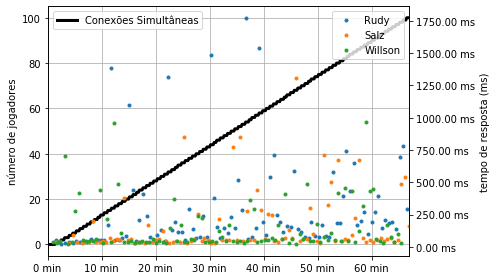
\includegraphics[width=0.8\textwidth]{figuras/analise/rt/create_account_operation_request_time.png}
  \centering

  Fonte: O próprio autor.
\end{figure}

Porém, existe, visivelmente, na Figura~\ref{fig:create_account_operation_request_time} uma disparidade entre dados em relação a arquitetura utilizada.
%
Esta disparidade exibe poucos pontos demorando muito para executar a operação de criação de conta.

Dado o contexto, o único recurso compartilhado com microsserviços que recebem conexões concorrentes é o acesso aos dados da arquitetura.
%
Tal acesso é dado diretamente aos bancos de dados Redis e PostgreSQL ou, no caso da arquitetura Rudy, pelo microsserviço \textit{rcrud}.
%
Nesse sentido, existe pela natureza da formação dos serviços uma diferença no tempo de resposta perceptível aos clientes.

Para quantificar a Figura~\ref{fig:create_account_operation_request_time}, faz sentido buscar os valores de média, variância, máximo e mínimo dos dados obtidos.
%
A Tabela~\ref{tab:create_account_operation_request_time} exibe estes valores estatísticos.

\begin{table}[htb!]
\centering
\begin{adjustbox}{max width=\textwidth}
\caption{Média, Variância, Máximo e Mínimo da operação Criar Conta}
\label{tab:create_account_operation_request_time}
\begin{tabular}{l|l|l|l|l}
\hline \hline
Arquitetura & Média     & Variância & Máximo    & Mínimo  \\ \hline \hline
Rudy        & 263,09 ms & 115701,29 & 1774,0 ms & 19,0 ms \\ \hline
Salz        & 152,53 ms & 50575,35  & 1304,0 ms & 28,0 ms \\ \hline
Willson     & 135,98 ms & 30573,78  & 968,0 ms  & 20,0 ms \\ \hline \hline
\end{tabular}

\end{adjustbox}
\end{table}
%ccm Notação decimal brasileira 

Como exibido na Tabela~\ref{tab:create_account_operation_request_time}, pode-se perceber que existe uma diferença abrupta na média de tempo de resposta da \ac{api} e na variância.
%
Os valores de máximo e mínimo somente são exibidos como pontos de atenção, entretanto como visível na Figura~\ref{fig:create_account_operation_request_time}, são poucas requisições que estrapolam a região de maior densidade de requisições, justificando uma grande variância.

No contexto do atual trabalho, pode-se assumir a variância como disparidade entre os dados.
%
Quanto maior o valor, mais instável é o tempo de resposta de determinada operação ao serviço, entretanto esta mesmo sendo instável tenderá a responder em uma média de tempo.

A partir deste contexto, pode-se definir que a média de tempo de resposta do serviço, ao criar uma nova conta, segue a seguinte relação:

$$
  \overline{CriarConta_{w}} < \overline{CriarConta_{s}} < \overline{CriarConta_{r}}
$$

Deste modo, entende-se:

\begin{itemize}
 \item $\overline{CriarConta_{r}}$: Tempo de resposta médio da operação criar conta na arquitetura Rudy;
 \item $\overline{CriarConta_{r}}$: Tempo de resposta médio da operação criar conta na arquitetura Salz; e
 \item $\overline{CriarConta_{r}}$: Tempo de resposta médio da operação criar conta na arquitetura Willson.
\end{itemize}

Dessa forma, pode-se dizer que para a operação de criar conta, em média, do ponto de vista de tempo de resposta, a arquitetura Willson é superior a arquitetura Salz e Rudy, respectivamente.
%
Também pode-se afirmar que a estabilidade desta operação, do ponto de vista de tempo de resposta, também segue a mesma sequência.
%ccm Indentificou melhor mas não justificou a origem dessa melhora

\subsubsection{Criar personagem}
\label{sec:op_create_char}

A operação de criar de personagem é efetuada sobre o protocolo \ac{tcp}/\ac{http}.
%
Nesta operação, o cliente envia um formulário em formato \ac{json} com informações básicas comuns em jogos \ac{mmorpg} para uma instância de personagem e dados de autenticação da conta.
%
Os dados são validados e inseridos no banco de dados, caso a validação esteja correta.

\begin{figure}[htb!]
  \caption{Tempo de resposta para criar personagens}
  \label{fig:create_character_operation_request}
  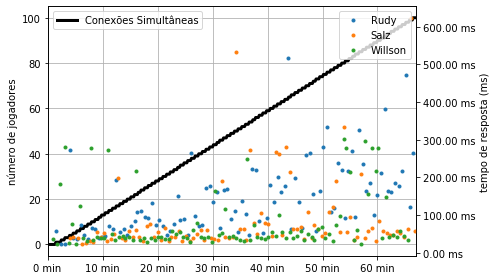
\includegraphics[width=0.8\textwidth]{figuras/analise/rt/create_character_operation_request.png}
  \centering

  Fonte: O próprio autor.
\end{figure}

Como pode-se perceber através da Figura~\ref{fig:create_character_operation_request}, o comportamento do tempo de resposta da perspectiva do cliente tem comportamento similar a operação criar conta (Subseção~\ref{sec:op_create_account}).
%
Nesse sentido, faz sentido aplicar o mesmo método de análise para validar se existem comportamentos similares, haja vista que a natureza desta operação é próxima.

Seguindo o método da média dos dados obtidos, pode-se obter os valores de média, variância, máximo e mínimo.
%
É possível visualizar estes valores na Tabela~\ref{tab:create_character_operation_request}.

\begin{table}[htb!]
\centering
\begin{adjustbox}{max width=\textwidth}
\caption{Média, Variância, Máximo e Mínimo da operação Criar Personagem}
\label{tab:create_character_operation_request}
\begin{tabular}{l|l|l|l|l}
\hline \hline
Arquitetura & Média     & Variância & Máximo    & Mínimo  \\ \hline \hline
Rudy        & 135,43 ms & 8782,99 & 517,0 ms & 23,0 ms \\ \hline
Salz        & 82,48 ms & 9106,62  & 624,0 ms & 24,0 ms \\ \hline
Willson     & 73,66 ms & 4886,60  & 301,0 ms  & 22,0 ms \\ \hline \hline
\end{tabular}

\end{adjustbox}

Fonte: O próprio autor.
\end{table}

A partir da Tabela~\ref{tab:create_character_operation_request}, pode-se observar que a média dos valores seguem o comportamento encontrado na operação Criar Conta (Subseção~\ref{sec:op_create_account}). 
%
Entretanto, é notório a diferença com relação a estabilidade da operação de criação de personagem.

Para realizar esta operação, o serviço realiza diversas validações, geralmente realizando a troca de mensagens entre os microsserviços de autenticação e validações de campos.
%
Tal situação, diferente da operação Criar Conta (Subseção~\ref{sec:op_create_account}), realiza poucas validações lógicas de regra de negócio aplicando-as diretamente ao banco de dados PostgreSQL.

A partir desta característica, pode-se analisar a diferença na estabilidade entre as arquiteturas Rudy e Salz.
%
Por mais que a arquitetura Salz seja melhor em média - do ponto de vista de tempo de resposta - comparada a arquitetura Rudy, a arquitetura Rudy possui uma maior estabilidade em seu tempo de resposta.
%
Tal estabilidade é proveniente do enfileiramento das requisições no microsserviço \textit{rcrud}.

Mesmo existindo uma flutuação maior na arquitetura Salz, nota-se que seus pontos máximos de tempo de resposta são inferiores aos da arquitetura Rudy.
%
Nesse sentido, por mais que o tempo de resposta tenha uma maior flutuação na arquitetura Salz, a arquitetura Rudy entrega uma menor qualidade.
%
Nesse sentido, deduz-se a seguinte relação:

$$
  \overline{CriarPersonagem_{w}} < \overline{CriarPersonagem_{s}} <\overline{CriarPersonagem_{r}}
$$

Onde entende-se:

\begin{itemize}
 \item $\overline{CriarPersonagem_{r}}$: Tempo de resposta médio da operação criar personagem na arquitetura Rudy;
 \item $\overline{CriarPersonagem_{s}}$: Tempo de resposta médio da operação criar personagem na arquitetura Salz; e
 \item $\overline{CriarPersonagem_{w}}$: Tempo de resposta médio da operação criar personagem na arquitetura Willson.
\end{itemize}

Esta relação também expressa a qualidade de serviço, do ponto de vista de tempo de resposta, entregue ao usuário, haja vista que a variação dos valores entre as arquiteturas Salz e Rudy são relevantes estatisticamente.
%
Porém, com uma magnitude baixa para utilizar como um argumento válido.
%
Dessa forma, entende-se que a arquitetura que entrega a melhor qualidade de serviço é a Willson, seguida pelas arquiteturas Salz e Rudy, respectivamente.



\subsubsection{Iniciar sessão}
\label{sec:op_start_session}
A operação de iniciar sessão é efetuada sobre o protocolo \ac{tcp}/\ac{rpc}.
%
Nesta operação, o cliente envia um formulário em formato \ac{gob} com informações básicas comuns em jogos \ac{mmorpg} para uma instância de personagem e dados de autenticação da conta.
%
Os dados são validados e o serviço retorna um dado assinado e armazenado para garantir a uniquicidade da sessão da conta.

\begin{figure}[htb!]
  \caption{Tempo de resposta para iniciar sessões}
  \label{fig:start_session_request_time}
  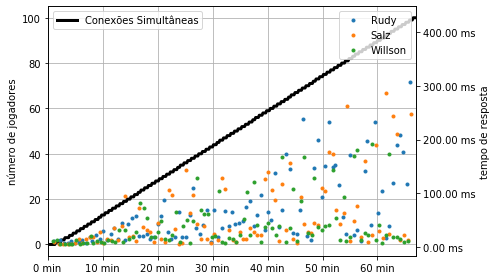
\includegraphics[width=0.8\textwidth]{figuras/analise/rt/start_session_request_time.png}
  \centering

  Fonte: O próprio autor.
\end{figure}

Tal qual as análises realizadas sobre as operações Criar Conta (Subseção~\ref{sec:op_create_account}) e Criar Personagem (Subseção~\ref{sec:op_create_char}), a Figura~\ref{fig:start_session_request_time} exibe tempo de requisições que foram realizadas somente uma vez por cliente.
%
Entretanto, o tempo de resposta está crescendo linearmente conforme o crescimento dos jogadores, diferente das outras operações.

A partir dessa diferença de comportamento, faz sentido analisar se existe algum crescimento, baseado na diluição destes dados a valores mais significativos para comparação.
%
Nesse contexto, faz sentido analisar o crescimento da média ao dividir as requisições em quadrantes.
%
Estes valores são exibidos na Tabela~\ref{tab:op_start_session}.

\begin{table}[htb!]
\centering
\begin{adjustbox}{max width=\textwidth}
\caption{Tempo de resposta médio dos quadrantes.}
\label{tab:op_start_session}
\begin{tabular}{l|l|l|l}

\hline \hline

Quadrante & Rudy    & Salz    & Willson \\ \hline \hline

Primeiro  & 18,6 ms & 20,88 ms & 15,68 ms \\ \hline

Segundo   & 45,4 ms & 52,38 ms & 40,48 ms \\ \hline

Terceiro  & 86,92 ms & 70,88 ms & 55,04 ms \\ \hline

Quarto    & 113,24 ms & 57,04 ms & 55,48 ms \\ \hline \hline

\end{tabular}

\end{adjustbox}

Fonte: O próprio autor.
\end{table}

A Tabela~\ref{tab:op_start_session} exibe o comportamento de crescimento conforme o crescimento de número de usuários, entretanto a média no último quadrante não aumenta proporcionalmente como nos quadrantes anteriores.
%
Não se pode, dessa forma, dizer que o crescimento é linear.

Outra informação exibida na Tabela~\ref{tab:op_start_session} é que a arquitetura Salz diminui drasticamente a média do seu tempo de resposta no quarto quadrante.
%
Também tem-se um incremento reduzido, se comparado aos demais quadrantes, quando visualiza-se o crescimento do quarto quadrante da arquitetura Willson.
%
Nesse sentido, o pode-se adicionar a variável de estabilidade da \ac{api} analisada.

Para realizar a análise de estabilidade, faz sentido buscar a variância dos dados de cada quadrante.
%
Dessa forma pode-se analisar se existe uma flutuação maior comparado aos quadrantes anteriores, mesmo com uma média próxima.
%
A Tabela~\ref{tab:op_start_session_var} exibe a variância dos quadrantes.


\begin{table}[htb!]
\centering
\begin{adjustbox}{max width=\textwidth}
\caption{Variância dos quadrantes na operação Iniciar Sessão.}
\label{tab:op_start_session_var}
\begin{tabular}{l|l|l|l}

\hline \hline

Quadrante & Rudy    & Salz    & Willson \\ \hline \hline

Primeiro  & 205,92 & 865,47 & 247,58 \\ \hline

Segundo   & 477,60 & 1138,57 & 960,09 \\ \hline

Terceiro  & 2785,59 & 4091,28 & 2307,08 \\ \hline

Quarto    & 4801,06 & 5192,71 & 3740,09 \\ \hline \hline

\end{tabular}

\end{adjustbox}

Fonte: O próprio autor.
\end{table}

A Tabela~\ref{tab:op_start_session_var} exibe a informação referente a variação dos dados nos quadrantes.
%
Dessa forma, pode-se afirmar que a variação aumenta conforme a carga do serviço aumenta.
%
Nesse sentido, por mais que a média não apresente comportamento linear, este comportamento linear existe, onde o mesmo é expresso pelo comportamento da variância.
%
Porém, a qualidade de serviço está expresso aos valores médios, e não a variação, a qual única e exclusivamente neste caso somente exibe o comportamento dos dados.
%
Dessa forma, deduz-se a seguinte relação:

$$
  \overline{IniciarSessao_{s}} < \overline{IniciarSessao_{w}} <\overline{IniciarSessao_{r}}
$$

Na qual entende-se:

\begin{itemize}
 \item $\overline{IniciarSessao_{r}}$: Tempo de resposta médio da operação iniciar sessão na arquitetura Rudy;
 \item $\overline{IniciarSessao_{s}}$: Tempo de resposta médio da operação iniciar sessão na arquitetura Salz; e
 \item $\overline{IniciarSessao_{w}}$: Tempo de resposta médio da operação iniciar sessão na arquitetura. Willson;
\end{itemize}
%ccm 13

\subsubsection{Instanciar personagem}

A operação de instanciar personagem é efetuada sobre o protocolo \ac{tcp}/\ac{rpc}.
%
Nesta operação, o cliente envia um formulário em formato \ac{gob} com informações de autenticação assinadas pelo serviço junto a informação de qual personagem deve ser instanciado no mundo virtual.
%
Os dados são validados e o personagem selecionado é instanciado no mundo.

\begin{figure}[htb!]
  \caption{Tempo de resposta para instanciar personagens}
  \label{fig:spawn_character_request_time}
  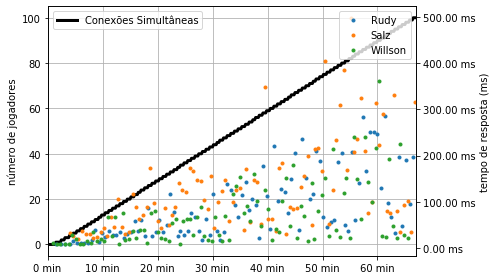
\includegraphics[width=0.8\textwidth]{figuras/analise/rt/spawn_character_request_time.png}
  \centering

  Fonte: O próprio autor.
\end{figure}

A Figura~\ref{fig:spawn_character_request_time} exibe o mesmo comportamento da operação iniciar sessão, abordada na Subseção~\ref{sec:op_start_session}.
%
Faz sentido aplicar os mesmos métodos para obter informação neste contexto, obtendo os valores de média e variância por quadrante.
%
Tais informações são exibidas na Tabela~\ref{tab:op_spawn_character}.

\begin{table}[htb!]
\centering
\begin{adjustbox}{max width=\textwidth}
\caption{Tempo de resposta médio e variância dos quadrantes para instanciar personagem.}
\label{tab:op_spawn_character}
\begin{tabular}{l||l|l||l|l||l|l}

\hline \hline

Quadrante & \multicolumn{2}{l||}{Rudy}    & \multicolumn{2}{l||}{Salz}    & \multicolumn{2}{l}{Willson} \\ \hline \hline

& Média & Variância & Média & Variância & Média & Variância \\ \hline

Primeiro  & 25,00 ms & 209,04 & 56,92 ms & 1350,23 & 24,64 ms & 368,15 \\ \hline

Segundo  & 59,12 ms & 1244,59 & 107,00 ms & 1617,25 & 42,24 ms & 8616,81 \\ \hline

Terceiro  & 123,00 ms & 3250,48 & 138,29 ms & 8661,54 & 86,72 ms & 2331,48 \\ \hline

Quarto  & 143.56 ms & 6984.89 & 202.12 ms & 14807.94 & 118.56 ms & 8616.81 \\ \hline \hline

\end{tabular}

\end{adjustbox}

Fonte: O próprio autor.
\end{table}

Diferente do comportamento da operação Iniciar Sessão (Subseção~\ref{sec:op_start_session}), ambos os comportamentos de variação e média exibidos na Tabela~\ref{tab:op_spawn_character} seguem um comportamento linear.
%
Deduz dessa forma que:

$$
  \overline{InstanciarPersonagem_{w}} < \overline{InstanciarPersonagem_{r}} <\overline{InstanciarPersonagem_{s}}
$$

No qual entende-se:

\begin{itemize}
 \item $\overline{InstanciarPersonagem_{r}}$: Tempo de resposta médio da operação instanciar personagem na arquitetura Rudy;
 \item $\overline{InstanciarPersonagem_{s}}$: Tempo de resposta médio da operação instanciar personagem na arquitetura Salz; e
 \item $\overline{InstanciarPersonagem_{w}}$: Tempo de resposta médio da operação instanciar personagem na arquitetura Willson.
\end{itemize}


\subsubsection{Movimentar personagem}

A operação de movimentar personagem é efetuada sobre o protocolo \ac{tcp}/\ac{rpc}.
%
Nesta operação, o cliente envia um formulário em formato \ac{gob} com informações de autenticação assinadas pelo serviço junto a um vetor de direção para onde o personagem deve caminhar no mundo virtual.
%
Os dados são validados e o personagem instanciado é movimentado.

\begin{figure}[htb!]
  \caption{Tempo de resposta para movimentar personagens}
  \label{fig:move_character_request_time}
  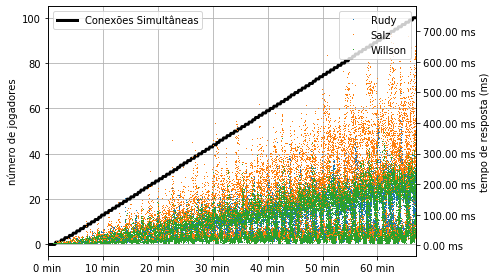
\includegraphics[width=0.8\textwidth]{figuras/analise/rt/move_character_request_time}
  \centering

  Fonte: O próprio autor.
\end{figure}

A Figura~\ref{fig:move_character_request_time} exibe os dados obtidos de tempo de resposta ao movimentar o personagem instanciado no \textit{chat} durante a variação do número de jogadores simultâneos.
%
Percebe-se um gráfico denso, dada a quantidade de pontos obtidos nos testes.
%
Dessa forma, faz sentido analisar o comportamento médio por jogador simultâneo.
%
A Figura~\ref{fig:spawn_character_request_time_per_concurrency} exibe o comportamento médio por jogador.

\begin{figure}[htb!]
  \caption{Tempo médio de resposta para movimentar personagem comparado ao número de jogadores}
  \label{fig:spawn_character_request_time_per_concurrency}
  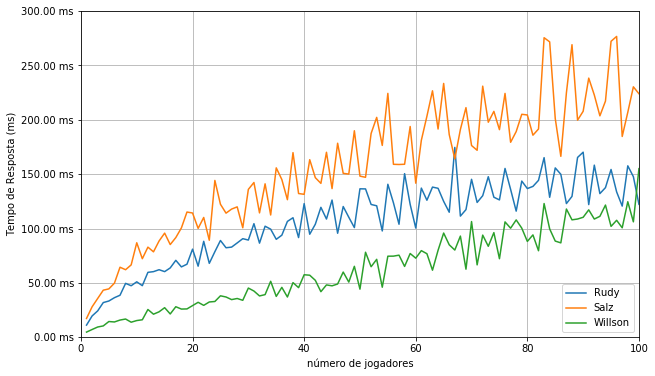
\includegraphics[width=0.8\textwidth]{figuras/analise/rt/spawn_character_request_time_per_concurrency}
  \centering

  Fonte: O próprio autor.
\end{figure}

Visivelmente, a Figura~\ref{fig:spawn_character_request_time_per_concurrency} permite deduzir dessa forma que:

$$
  \overline{MoverPersonagem_{w}} < \overline{MoverPersonagem_{r}} <\overline{MoverPersonagem_{s}}
$$

No qual entende-se:

\begin{itemize}
 \item $\overline{MoverPersonagem_{r}}$: Tempo de resposta médio da operação mover personagem na arquitetura Rudy;
 \item $\overline{MoverPersonagem_{s}}$: Tempo de resposta médio da operação mover personagem na arquitetura Salz; e
 \item $\overline{MoverPersonagem_{w}}$: Tempo de resposta médio da operação mover personagem na arquitetura Willson.
\end{itemize}


\subsubsection{Enviar mensagem}

A operação de enviar mensagem é efetuada sobre o protocolo \ac{tcp}/\ac{rpc}.
%
Nesta operação, o cliente envia um formulário em formato \ac{gob} com informações de autenticação assinadas pelo serviço junto a uma linha de texto.
%
Os dados são validados e a linha de texto é distribuído aos personagens dentro do raio de visão do personagem emissor instanciado.

\begin{figure}[htb!]
  \caption{Tempo de resposta para enviar mensagens}
  \label{fig:send_chat_request_time}
  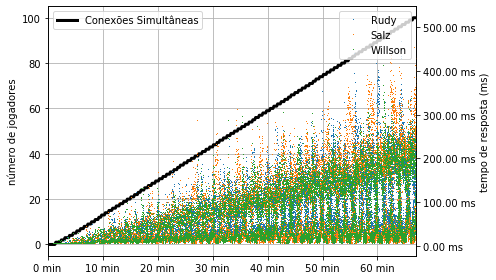
\includegraphics[width=0.8\textwidth]{figuras/analise/rt/send_chat_request_time}
  \centering

  Fonte: O próprio autor.
\end{figure}

A Figura~\ref{fig:send_chat_request_time} exibe os dados obtidos de tempo de resposta ao enviar uma mensagem no chat durante a variação do número de jogadores simultâneos.
%
Percebe-se um gráfico denso, dada a quantidade de pontos obtidos nos testes.
%
Dessa forma, faz sentido analisar o comportamento médio por jogador simultâneo.
%
A Figura~\ref{fig:send_chat_request_time_per_concurrency} exibe o comportamento médio por jogador.


\begin{figure}[htb!]
  \caption{Tempo médio de resposta para enviar mensagens comparado ao número de jogadores}
  \label{fig:send_chat_request_time_per_concurrency}
  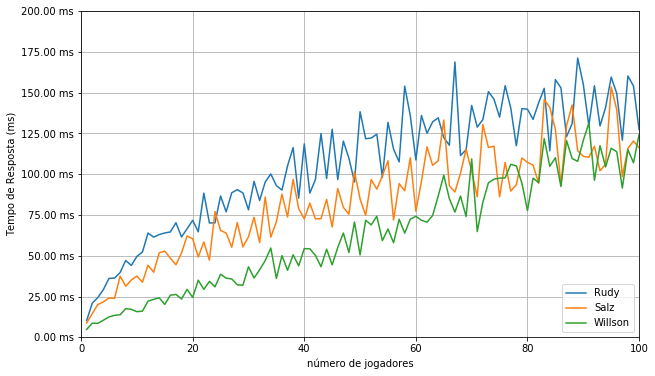
\includegraphics[width=0.8\textwidth]{figuras/analise/rt/send_chat_request_time_per_concurrency}
  \centering

  Fonte: O próprio autor.
\end{figure}

Visivelmente, a Figura~\ref{fig:send_chat_request_time_per_concurrency} permite deduzir dessa forma que:

$$
  \overline{EnviarMensagem_{w}} < \overline{EnviarMensagem_{s}} <\overline{EnviarMensagem_{r}}
$$

No qual entende-se:

\begin{itemize}
 \item $\overline{EnviarMensagem_{r}}$: Tempo de resposta médio da operação enviar mensagem na arquitetura Rudy;
 \item $\overline{EnviarMensagem_{s}}$: Tempo de resposta médio da operação enviar mensagem na arquitetura Salz; e
 \item $\overline{EnviarMensagem_{w}}$: Tempo de resposta médio da operação enviar mensagem na arquitetura Willson.
\end{itemize}

\subsubsection{Receber mensagem}

A operação de receber mensagem é efetuada sobre o protocolo \ac{tcp}/\ac{rpc}.
%
Nesta operação, o cliente envia um formulário em formato \ac{gob} com informações de autenticação assinadas pelo serviço.
%
Os dados são validados e o serviço retorna todas as linhas de texto que foram encaminhadas ao personagem instanciado.

\begin{figure}[htb!]
  \caption{Tempo de resposta para receber mensagens}
  \label{fig:listen_chat_request_time}
  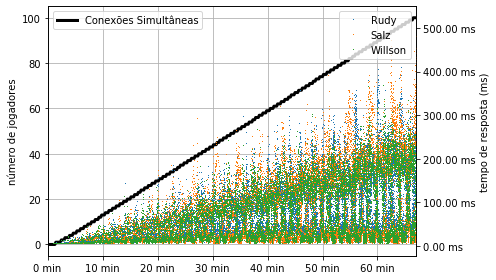
\includegraphics[width=0.8\textwidth]{figuras/analise/rt/listen_chat_request_time}
  \centering

  Fonte: O próprio autor.
\end{figure}

A Figura~\ref{fig:listen_chat_request_time} exibe os dados obtidos de tempo de resposta ao receber uma mensagem no chat durante a variação do número de jogadores simultâneos.
%
Percebe-se um gráfico denso, dada a quantidade de pontos obtidos nos testes.
%
Dessa forma, faz sentido analisar o comportamento médio por jogador simultâneo.
%
A Figura~\ref{fig:listen_chat_request_time_per_concurrency} exibe o comportamento médio por jogador.

\begin{figure}[htb!]
  \caption{Tempo médio de resposta para receber mensagens comparado ao número de jogadores}
  \label{fig:listen_chat_request_time_per_concurrency}
  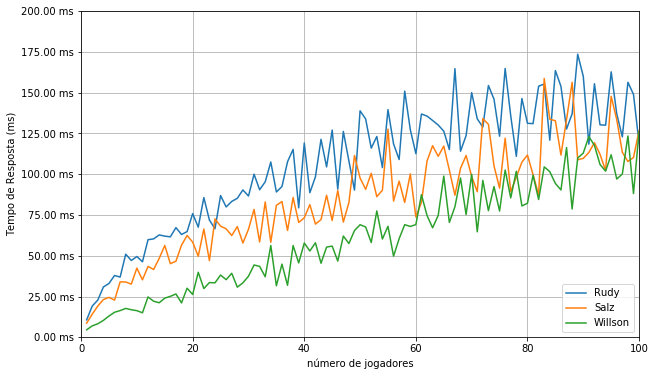
\includegraphics[width=0.8\textwidth]{figuras/analise/rt/listen_chat_request_time_per_concurrency}
  \centering

  Fonte: O próprio autor.
\end{figure}

Visivelmente, a Figura~\ref{fig:listen_chat_request_time_per_concurrency} permite deduzir dessa forma que:

$$
  \overline{ReceberMensagem_{w}} < \overline{ReceberMensagem_{s}} <\overline{ReceberMensagem_{r}}
$$

Onde entende-se:

\begin{itemize}
 \item $\overline{ReceberMensagem_{r}}$: Tempo de resposta médio da operação receber mensagem na arquitetura Rudy;
 \item $\overline{ReceberMensagem_{s}}$: Tempo de resposta médio da operação receber mensagem na arquitetura Salz; e
 \item $\overline{ReceberMensagem_{w}}$: Tempo de resposta médio da operação receber mensagem na arquitetura Willson.
\end{itemize}

\subsection{Consumo de \ac{cpu}}

Este experimento visa analisar o consumo de \ac{cpu} unitariamente, em relação ao número de jogadores simultâneos.
%
Espera-se que o seu crescimento seja de tendência linear junto ao crescimento de jogadores concorrentes.
%
Neste contexto existem os seguintes valores:

\begin{itemize}
    \item Jogadores simultâneos: Variável capturada a partir do microsserviço de jogo; e
    \item Consumo de \ac{cpu}: Variável capturada a partir do monitor de recursos do Docker.
\end{itemize}

Nota-se que o número de jogadores simultâneos e o consumo de \ac{cpu} são indexados pelo tempo a qual tais dados foram capturados.
%
Nesse sentido, pode-se relacionar o número de jogadores simultâneos ao consumo de \ac{cpu} dos microsserviços e do banco de dados.
%
Dado tal contexto, faz sentido realizar uma análise separando os ambientes de Banco de Dados de Microsserviços.

\subsubsection{Banco de Dados}

Considerando o ambiente de banco de dados, pode-se realizar a associação de número de jogadores simultâneos e \ac{cpu} consumida pelos contêineres de banco de dados.
%
Essa associação é realizada pelo tempo de registro das métricas.
%
O resultado desta associação pode ser visualizado na Figura~\ref{fig:experimento_db_cpu}.



\begin{figure}[htb!]
    \caption{Consumo de \ac{cpu} dos bancos de dados}
    \label{fig:experimento_db_cpu}

    \begin{subfigure}{0.5\textwidth}
        \centering
        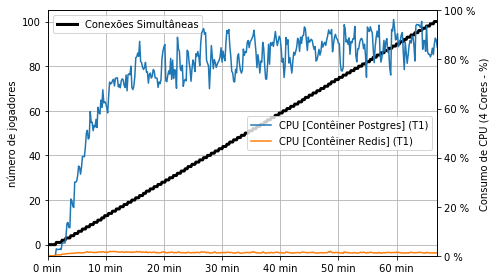
\includegraphics[width=.95\linewidth]{figuras/testes/r_cpu_db.png}
        \caption{Bancos de Dados da arquitetura Rudy}
        \label{fig:r_cpu_db}
    \end{subfigure}%
    \begin{subfigure}{0.5\textwidth}
        \centering
        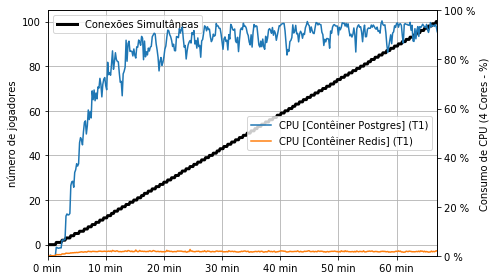
\includegraphics[width=.95\linewidth]{figuras/testes/s_cpu_db.png}
        \caption{Bancos de Dados da arquitetura Salz}
        \label{fig:s_cpu_db}
    \end{subfigure}\\

    \begin{subfigure}{0.5\textwidth}
        \centering
        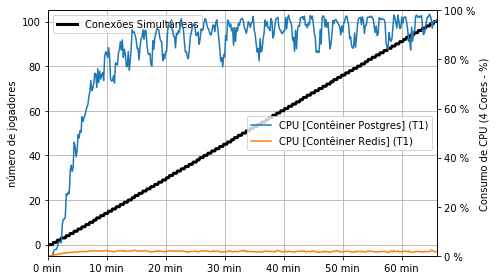
\includegraphics[width=.95\linewidth]{figuras/testes/w_cpu_db.png}
        \caption{Bancos de Dados da arquitetura Willson}
        \label{fig:w_cpu_db}
    \end{subfigure}

    Fonte: O próprio autor.
\end{figure}


A Figura~\ref{fig:experimento_db_cpu} exibe o comportamento do consumo de \ac{cpu} durante a execução dos testes para as arquiteturas Rudy (Subfigura~\ref{fig:r_cpu_db}), Salz (Subfigura~\ref{fig:s_cpu_db}) e Willson (Subfigura~\ref{fig:w_cpu_db}).
%
Em todas as figuras é notório o seguinte comportamento:

\begin{itemize}
 \item Baixo consumo de \ac{cpu} do servidor de dados temporários (Redis), com comportamento linear estável; e
 \item Alto consumo de \ac{cpu} do servidor de dados permanentes (PostgreSQL), com comportamento multimodal.
\end{itemize}

Este comportamento era esperado, dado a natureza distinta de ambos os banco de dados, na qual PostgreSQL é um banco de dados \ac{acid} e o Redis é um banco de dados \ac{nosql}.
%
Entretanto, é notório a discrepância entre ambos os bancos de dados, afimando-se que o banco de dados temporário é estável em relação ao consumo de \ac{cpu}.

Ao analisar o comportamento do banco de dados persistentes para as arquiteturas Rudy (Subfigura~\ref{fig:r_cpu_db}), Salz (Subfigura~\ref{fig:s_cpu_db}) e Willson (Subfigura~\ref{fig:w_cpu_db}) observamos um comportamento diferente na arquitetura Rudy.
%
Dada esta percepção, faz sentido analisar a tendência destas curvas com base em sua média.
%
A Tabela~\ref{tab:cpu_db_media_quadrantes} exibe os valores das médias baseado em todo o decorrer do experimento e dividindo o experimento em quadrantes.

\begin{table}[htb!]
\centering
\begin{adjustbox}{max width=\textwidth}
\caption{Consumo de \ac{cpu} por quadrante pelo PostgreSQL.}
\label{tab:cpu_db_media_quadrantes}
\begin{tabular}{l|l|l|l}

\hline \hline

Quadrante & Rudy    & Salz    & Willson \\ \hline \hline

Primeiro  & 50,60\% & 53,10\% & 58,15\% \\ \hline

Segundo   & 80,66\% & 88,04\% & 89,86\% \\ \hline

Terceiro  & 85,61\% & 90,77\% & 92,50\% \\ \hline

Quarto    & 86,94\% & 92,07\% & 93,48\% \\ \hline \hline

\end{tabular}

\end{adjustbox}

Fonte: O próprio autor.
\end{table}

Torna-se visível a diferença do consumo de \ac{cpu} entre as arquiteturas pelo banco de dados.
%
A partir destes dados pode-se deduzir que:

\begin{itemize}
 \item Arquitetura Rudy consome menos \ac{cpu} do banco de dados persistentes; e 
 \item Arquitetura Salz e Willson consomem \ac{cpu} na mesma proporção, com a arquitetura Salz tendo uma leva tendência a consumir menos \ac{cpu}.
\end{itemize}

Para tornar esta diferença visível ao longo de toda a progressão da carga, faz sentido exibir esta informação em um gráfico de linha.
%
A Figura~\ref{fig:cpu_db_media_por_jogador} exibe a média de consumo de \ac{cpu} pelo contêiner PostgreSQL comparado ao número de jogadores simultâneos.

\begin{figure}[htb!]
  \caption{Consumo de \ac{cpu} pelo PostgreSQL comparado ao número de jogadores simultâneos.}
  \label{fig:cpu_db_media_por_jogador}
  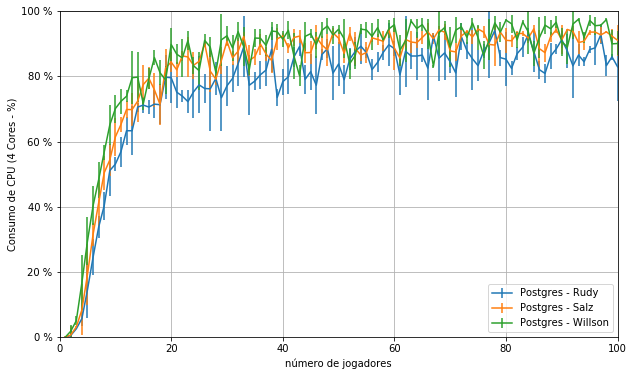
\includegraphics[width=0.8\textwidth]{figuras/analise/cpu_db_media_por_jogador.png}
  \centering

  Fonte: O próprio autor.
\end{figure}

Conforme exibido na Figura~\ref{fig:cpu_db_media_por_jogador}, pode-se deduzir que em todo caso as arquiteturas Rudy, Salz e Willson seguem a seguinte expressão:

$$
    CPU(db\_postgresql_{r}) < CPU(db\_postgresql_{s}) \approx CPU(db\_postgresql_{w})
$$

Na qual entende-se:

\begin{itemize}
\item $CPU(db\_postgresql_{r})$: Curva de consumo de \ac{cpu} pelo PostgreSQL da arquitetura Rudy;
\item $CPU(db\_postgresql_{s})$: Curva de consumo de \ac{cpu} pelo PostgreSQL da arquitetura Salz; e
\item $CPU(db\_postgresql_{w})$: Curva de consumo de \ac{cpu} pelo PostgreSQL da arquitetura Willson.
\end{itemize}

O banco de dados temporários consome pouca \ac{cpu}, comparado ao banco de dados persistentes.
%
Entretanto, faz sentido realizar a mesma análise para validar se existe alguma diferença no seu uso conforme a arquitetura empregada.
%
Dessa forma, foi dividido em quadrantes para analisar o consumo médio de \ac{cpu}, a qual é exibido na Tabela~\ref{tab:cpu_redis_media_quadrantes}.

\begin{table}[htb!]
\centering
\begin{adjustbox}{max width=\textwidth}
\caption{Consumo de \ac{cpu} por quadrante pelo Redis.}
\label{tab:cpu_redis_media_quadrantes}
\begin{tabular}{|l|l|l|l|}

\hline

Quadrante & Rudy    & Salz    & Willson \\ \hline

Primeiro  & 1,24\% & 1,46\% & 1,60\% \\ \hline

Segundo   & 1,32\% & 1,79\% & 1,81\% \\ \hline

Terceiro  & 1,28\% & 1,75\% & 1,75\% \\ \hline

Quarto    & 1,26\% & 1,73\% & 1,72\% \\ \hline

\end{tabular}

\end{adjustbox}

Fonte: O próprio autor.
\end{table}

Dado os valores da Tabela~\ref{tab:cpu_redis_media_quadrantes}, pode-se obter as seguintes conclusões:

\begin{itemize}
 \item Rudy consome menos \ac{cpu} do banco de dados temporários; e
 \item A arquitetura Salz e Willson consomem \ac{cpu} com o mesmo comportamento.
\end{itemize}

Para tornar esta diferença visível ao longo de toda a progressão da carga, faz sentido exibir esta informação em um gráfico de linha.
%
A Figura~\ref{fig:cpu_redis_media_por_jogador} exibe um gráfico a qual compara a média de consumo de \ac{cpu} conforme o número de jogadores simultâneos.

\begin{figure}[htb!]
  \caption{Consumo de \ac{cpu} pelo PostgreSQL comparado ao número de jogadores simultâneos.}
  \label{fig:cpu_redis_media_por_jogador}
  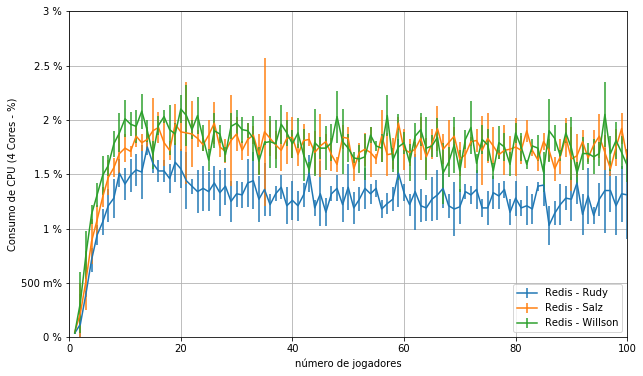
\includegraphics[width=0.8\textwidth]{figuras/analise/cpu_redis_media_por_jogador.png}
  \centering

  Fonte: O próprio autor.
\end{figure}

Conforme exibido na Figura~\ref{fig:cpu_redis_media_por_jogador}, pode-se deduzir que em todo caso as arquiteturas Rudy, Salz e Willson seguem a seguinte expressão:

$$
    CPU(db\_redis_{r}) < CPU(db\_redis_{s}) \approx CPU(db\_redis_{w})
$$

Na qual entende-se:

\begin{itemize}
\item $CPU(db\_redis_{r})$: Curva de consumo de \ac{cpu} pelo Redis da arquitetura Rudy;
\item $CPU(db\_redis_{s})$: Curva de consumo de \ac{cpu} pelo Redis da arquitetura Salz; e
\item $CPU(db\_redis_{w})$: Curva de consumo de \ac{cpu} pelo Redis da arquitetura Willson.
\end{itemize}

Nota-se que o consumo de recurso do banco de dados temporários e banco de dados persistentes exibiram o mesmo comportamento.
%
Dessa forma, pode-se generalizar o comportamento do consumo de \ac{cpu} das arquiteturas Rudy, Salz e Willson para banco de Dados:

$$
    CPU(db_{r}) < CPU(db_{s}) \approx CPU(db_{w})
$$

Na qual entende-se:

\begin{itemize}
\item $CPU(db_{r})$: Curva de consumo de \ac{cpu} pelos banco de dados da arquitetura Rudy;
\item $CPU(db_{s})$: Curva de consumo de \ac{cpu} pelos banco de dados da arquitetura Salz; e
\item $CPU(db_{w})$: Curva de consumo de \ac{cpu} pelos banco de dados da arquitetura Willson.
\end{itemize}

Este comportamento é dado pela característica do microsserviço \textit{rcrud} que realiza uma multiplexação de conexões entre o banco de dados e a arquitetura.
%
Entretanto, esta característica pode ser por dois motivos:

\begin{itemize}
 \item O banco de dados está otimizado para responder uma única conexão, consumindo menos \ac{cpu}; ou
 \item O banco de dados não consome tanta \ac{cpu} por ter um microsserviço que tornou-se um gargalo como frente do banco de dados.
\end{itemize}

Dado estas duas hipóteses, faz sentido mensurar a qualidade de serviço entregue ao usuário.
%
Pode-se mensurar qual das hipóteses é mais valiosa para a qualidade de serviço com base no tempo de resposta do usuário.


\subsubsection{Microsserviços}

Considerando o ambiente de banco de dados, pode-se realizar a associação de número de jogadores simultâneos e \ac{cpu} consumida pelos contêineres de banco de dados.
%
Essa associação é realizada pelo tempo de registro das métricas.
%
O resultado desta associação pode ser visualizado na Figura~\ref{fig:experimento_game_cpu}.

\begin{figure}[htb!]
    \caption{Consumo de \ac{cpu} dos microsserviços}
    \label{fig:experimento_game_cpu}

    \begin{subfigure}{0.5\textwidth}
        \centering
        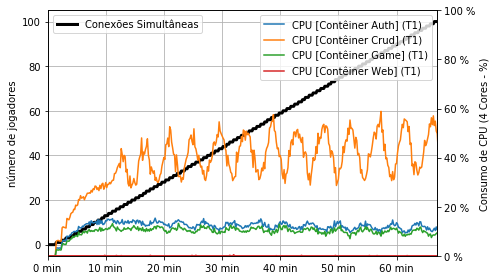
\includegraphics[width=.95\linewidth]{figuras/testes/r_cpu_game.png}
        \caption{Microsserviços da arquitetura Rudy}
        \label{fig:r_cpu_game}
    \end{subfigure}%
    \begin{subfigure}{0.5\textwidth}
        \centering
        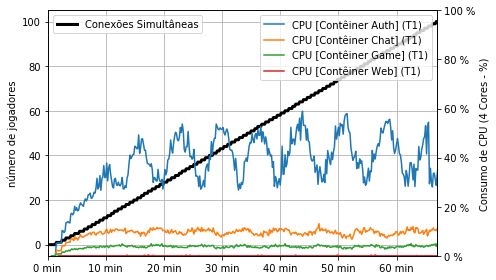
\includegraphics[width=.95\linewidth]{figuras/testes/s_cpu_game.png}
        \caption{Microsserviços da arquitetura Salz}
        \label{fig:s_cpu_game}
    \end{subfigure}

    \begin{subfigure}{0.5\textwidth}
        \centering
        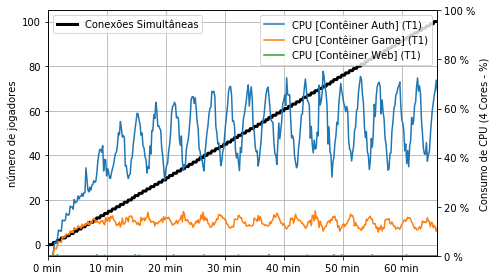
\includegraphics[width=.95\linewidth]{figuras/testes/w_cpu_game.png}
        \caption{Microsserviços da arquitetura Willson}
        \label{fig:w_cpu_game}
    \end{subfigure}%

    Fonte: O próprio autor.
\end{figure}

Conforme exibido nas Figuras~\ref{fig:r_cpu_game}, ~\ref{fig:s_cpu_game} e ~\ref{fig:w_cpu_game}, pode-se observar as seguintes características:

\begin{itemize}
 \item Os microsserviços \textit{rweb}, \textit{sweb} e \textit{wweb} consomem pouca \ac{cpu} comparado a todos os outros microsserviços das arquiteturas; e
 \item Os microsserviços \textit{rcrud}, \textit{sauth} e \textit{wauth} são os microsserviços que mais consomem \ac{cpu} nas arquiteturas Rudy, Salz e Willson.
\end{itemize}

Faz sentido analisar a média do consumo de \ac{cpu} dos microsserviços dividindo em quadrantes.
%
Dessa forma, pode-se obter dados significantes para realizar comparações a partir destes dados.
%
A Tabela~\ref{tab:cpu_microsservicos_media_quadrantes} exibe a média de consumo de \ac{cpu} por quadrante de todos os microsserviços.

\begin{table}[htb!]
\centering
\begin{adjustbox}{max width=\textwidth}
\caption{Consumo de \ac{cpu} por quadrante dos microsserviços.}
\label{tab:cpu_microsservicos_media_quadrantes}

\begin{tabular}{|l|l|l|l|l|}
\hline
Microsserviço & Primeiro Quadrante & Segundo Quadrante & Terceiro Quadrante & Quarto Quadrante \\ \hline
rauth         & 11,22\%            & 12,52\%           & 11,88\%            & 11,56\%          \\ \hline
rcrud         & 25,97\%            & 41,83\%           & 42,50\%             & 43,62\%          \\ \hline
rgame         & 8,92\%             & 10,54\%           & 10,14\%            & 9,58\%           \\ \hline
rweb          & 0,01\%             & 0,01\%            & 0,01\%             & 0,01\%           \\ \hline
sauth         & 26,08\%            & 39,95\%           & 43,22\%            & 40,96\%          \\ \hline
schat         & 8,34\%             & 9,97\%            & 9,59\%             & 9,61\%           \\ \hline
sgame         & 3,12\%             & 3,87\%            & 3,72\%             & 3,85\%           \\ \hline
sweb          & 0,01\%             & 0,01\%            & 0,01\%             & 0,01\%           \\ \hline
wauth         & 23,79\%            & 50,73\%           & 57,11\%            & 56,69\%          \\ \hline
wgame         & 9,68\%             & 14,20\%           & 13,66\%            & 13,42\%          \\ \hline
wweb          & 0,01\%             & 0,01\%            & 0,01\%             & 0,01\%           \\ \hline
\end{tabular}
\end{adjustbox}

Fonte: O próprio autor.
\end{table}

A Tabela~\ref{tab:cpu_microsservicos_media_quadrantes} mostra o crescimento do consumo de carga médio dos quadrantes.
%
Estes dados são importantes, haja vista que os mesmos permitem analisar o comportamento das curvas removendo oscilações notórias na visualização do consumo de \ac{cpu}.
%
A partir desta tabela pode-se realizar as seguintes conclusões:

\begin{itemize}
 \item Entre os microsserviços \textit{rcrud}, \textit{sauth} e \textit{wauth}, o com maior consumo é o microsserviço \textit{wauth}; e
 \item Os microsserviços \textit{rweb}, \textit{sweb} e \textit{wweb} possuem o mesmo consumo, em média.
\end{itemize}

É relevante, a partir destas conclusões, analisar a média em relação a progressão de usuários.
%
A visualização da média de consumo de \ac{cpu} por usuário simultâneo tem como objetivo remover ruídos que possam afetar a visualização dos dados.

\begin{figure}[htb!]
    \caption{Média do consumo de \ac{cpu} dos microsserviços por jogador simultâneo}
    \label{fig:cpu_game_media_por_jogador}

    \begin{subfigure}{0.5\textwidth}
        \centering
        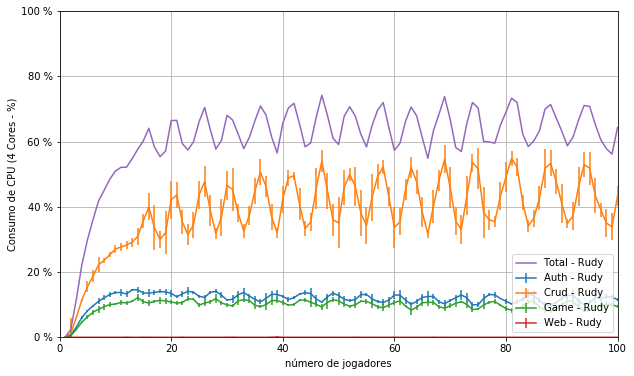
\includegraphics[width=.95\linewidth]{figuras/analise/cpu_r_arch_media_por_jogador.png}
        \caption{Microsserviços da arquitetura Rudy}
        \label{fig:cpu_r_arch_media_por_jogador}
    \end{subfigure}%
    \begin{subfigure}{0.5\textwidth}
        \centering
        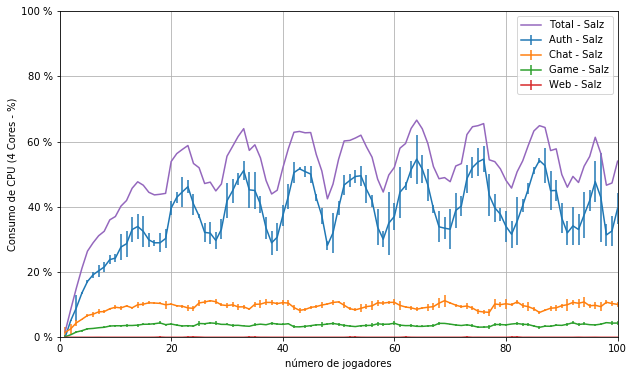
\includegraphics[width=.95\linewidth]{figuras/analise/cpu_s_arch_media_por_jogador.png}
        \caption{Microsserviços da arquitetura Salz}
        \label{fig:cpu_s_arch_media_por_jogador}
    \end{subfigure}

    \begin{subfigure}{0.5\textwidth}
        \centering
        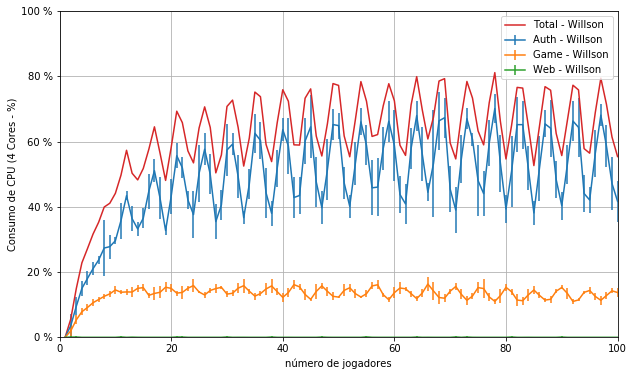
\includegraphics[width=.95\linewidth]{figuras/analise/cpu_w_arch_media_por_jogador.png}
        \caption{Microsserviços da arquitetura Willson}
        \label{fig:cpu_w_arch_media_por_jogador}
    \end{subfigure}%

    Fonte: O próprio autor.
\end{figure}

A Figura~\ref{fig:cpu_game_media_por_jogador} tem como objetivo exibir a média de consumo de \ac{cpu} por jogador, assim permitindo analisar o comportamento das curvas.
%
Entretanto, nota-se que todos os microsserviços contém uma característica senoidal, onde sua amplitude aumenta com a quantidade de jogadores, na qual já era visível na Figura~\ref{fig:experimento_game_cpu}.
%
Porém, neste gráfico também é visível o erro de cada média.
%
Este erro é dado pela variância do conjunto de dados obtidos na determinada faixa de jogadores simultâneos.
%
Ter um valor de variância alto significa que, por mais que a média seja um bom valor para a métrica, diversos pontos da mesma faixa estão longe deste valor.
%
Dessa forma, pode-se interpretar como um erro, neste contexto.

Pode-se deduzir as seguintes características a partir da Figura~\ref{fig:cpu_game_media_por_jogador}:

\begin{itemize}
 \item Os microsserviços que contém maior erro são os que estão relacionados a acesso de dados para autenticação ou/e geração de assinaturas de dados para outros serviços (\textit{rcrud, sauth e wauth});
 \item Os microsserviços que contém maior erro, são os que lideram a lista de maior consumo de \ac{cpu}, porém nota-se a partir dos demais microsserviços que esta relação não é proporcional a carga; e
 \item O valor total de consumo de \ac{cpu} mudou conforme a arquitetura.
\end{itemize}

Dado o último critério, utilizando a curva de total consumido das Sub figuras~\ref{fig:cpu_r_arch_media_por_jogador}, ~\ref{fig:cpu_s_arch_media_por_jogador} e ~\ref{fig:cpu_w_arch_media_por_jogador},  pode-se comparar o total de consumo de \ac{cpu} por cada arquitetura.
%
A Tabela~\ref{tab:consumo_total_cpu} exibe os valores baseados em quadrantes, para realizar a comparação com valores.


\begin{table}[htb!]
\centering
\begin{adjustbox}{max width=\textwidth}
\caption{Consumo total de \ac{cpu} por quadrante dos microsserviços.}
\label{tab:consumo_total_cpu}

\begin{tabular}{|l|l|l|l|l|}
\hline
Arquitetura & Primeiro Quadrante & Segundo Quadrante & Terceiro Quadrante & Quarto Quadrante \\ \hline
Rudy        & 47,05\%            & 64,51\%           & 65,25\%            & 64,31\%          \\ \hline
Salz        & 38,74\%            & 53,87\%           & 56,74\%            & 54,27\%          \\ \hline
Willson     & 44,60\%            & 65,76\%           & 67,94\%            & 66,98\%          \\ \hline
\end{tabular}
\end{adjustbox}

Fonte: O próprio autor.
\end{table}

A partir dos dados da Tabela~\ref{tab:consumo_total_cpu}, pode-se referenciar que a arquitetura Salz consome menos \ac{cpu} que a arquitetura Rudy e Willson.
%
Faz sentido realizar a visualização das três curvas de totais em um único gráfico a fim de exibir esta relação.
%
A Figura~\ref{fig:consumo_total_cpu} exibe esta comparação.

\begin{figure}[htb!]
  \caption{Comparação de consumo total de \ac{cpu} pelas arquiteturas.}
  \label{fig:consumo_total_cpu}
  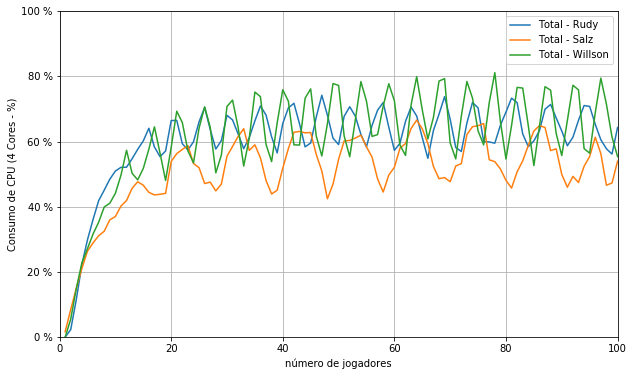
\includegraphics[width=0.8\textwidth]{figuras/analise/cpu_total_archs.png}
  \centering

  Fonte: O próprio autor.
\end{figure}

Dado a Figura~\ref{fig:consumo_total_cpu} e a Tabela~\ref{tab:consumo_total_cpu}, pode-se afirmar que:

$$
    CPU(microsservicos_{s}) < CPU(microsservicos_{r}) < CPU(microsservicos_{w})
$$

Na qual entende-se:

\begin{itemize}
\item $CPU(microsservicos_{r})$: Curva de consumo de \ac{cpu} pelos microsserviços da arquitetura Rudy;
\item $CPU(microsservicos_{s})$: Curva de consumo de \ac{cpu} pelos microsserviços da arquitetura Salz; e
\item $CPU(microsservicos_{w})$: Curva de consumo de \ac{cpu} pelos microsserviços da arquitetura Willson.
\end{itemize}

Torna-se notório que tal sequência respeita a ordem de interconexões dos microsserviços.
%
Nesse sentido, a arquitetura Salz possui mais conexões que a arquitetura Rudy, que possui mais conexões que a arquitetura Willson.

Nota-se, que possuir um consumo de \ac{cpu} maior que outra arquitetura não implica em ser uma arquitetura melhor.
%
Pode-se encontrar dois casos para um consumo de \ac{cpu} ao comparar duas arquiteturas:

\begin{itemize}
 \item A arquitetura possui pouca carga para estressar a \ac{cpu}; ou
 \item A arquitetura converge para tal valor, visto que está com gargalo em outro recurso necessário.
\end{itemize}

Para o caso desta análise, pode-se descartar a primeira alternativa.
%
Para este caso pode-se analisar que a curva estabiliza o seu crescimento entre 20 e 40 jogadores simultâneos, a mesma faixa na qual os bancos de dados estabilizaram seu crescimento (visível na Figura~\ref{fig:cpu_db_media_por_jogador}).
%
Dessa forma, pode-se justificar o aumento de erros nas médias nos microsserviços com acesso ao banco conforme o aumento da carga no serviço.

Outra característica das curvas obtidas é a frequência da oscilação encontrada, característica visível na Figura~\ref{fig:consumo_total_cpu}.
%
Nota-se que a frequência é escalada tal qual a crista de uma onda entra em contato com o vale da outra onda.
%
Tal característica das curvas não é coincidência, sendo resultado do escalonador de contêineres.
%
A Figura~\ref{fig:cpu_w_arch_media_por_jogador} é a que melhor exemplifica este comportamento, haja vista que a arquitetura Willson possui somente dois microsserviços que são impactados diretamente por este escalonador.


\subsection{Consumo de Memória}



Este experimento visa analisar o consumo de memória unitariamente, em relação ao número de jogadores simultâneos.
%
Espera-se que o seu crescimento seja linear seguindo o crescimento de jogadores concorrentes.
%
Neste contexto existem os seguintes valores:



\begin{itemize}
    \item Jogadores simultâneos: Variável capturada a partir do microsserviço de jogo; e
    \item Consumo de memória: Variável capturada a partir do monitor de recursos do Docker.
\end{itemize}

Nota-se que o número de jogadores simultâneos e o consumo de memória são indexados pelo tempo a qual tais dados foram capturados.
%
Nesse sentido, pode-se relacionar, o número de jogadores simultâneos ao consumo de memória dos microsserviços e do banco de dados.
%
Dado tal contexto, faz sentido realizar uma análise separando os ambientes de Banco de Dados de Microsserviços.

\subsubsection{Banco de Dados}



Considerando o ambiente de banco de dados, pode-se realizar a associação de número de jogadores simultâneos e memória consumida pelos contêineres de banco de dados.
%
Essa associação é realizada pelo tempo de registro das métricas.
%
O resultado desta associação pode ser visualizado na Figura~\ref{fig:experimento_db_mem}.



\begin{figure}[htb!]
    \caption{Consumo de memória dos bancos de dados}
    \label{fig:experimento_db_mem}

    \begin{subfigure}{0.5\textwidth}
        \centering
        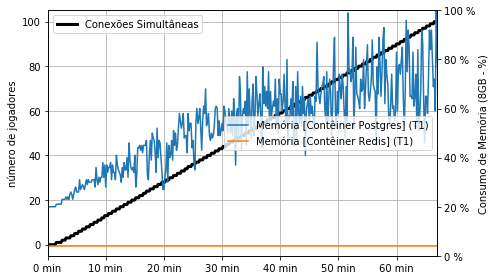
\includegraphics[width=.95\linewidth]{figuras/testes/r_mem_db.png}
        \caption{Bancos de Dados da arquitetura Rudy}
        \label{fig:r_mem_db}
    \end{subfigure}%
    \begin{subfigure}{0.5\textwidth}
        \centering
        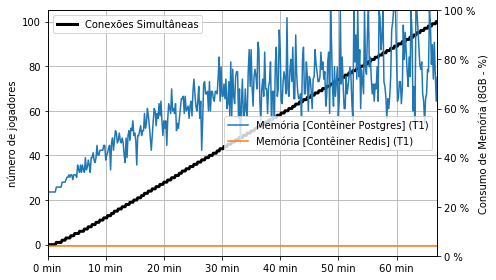
\includegraphics[width=.95\linewidth]{figuras/testes/s_mem_db.png}
        \caption{Bancos de Dados da arquitetura Salz}
        \label{fig:s_mem_db}
    \end{subfigure}\\

    \begin{subfigure}{0.5\textwidth}
        \centering
        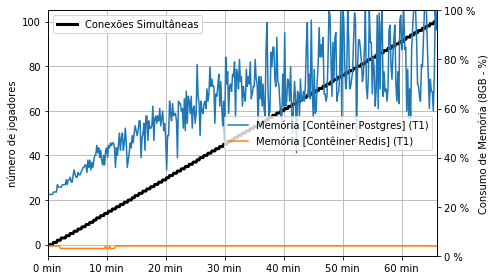
\includegraphics[width=.95\linewidth]{figuras/testes/w_mem_db.png}
        \caption{Bancos de Dados da arquitetura Willson}
        \label{fig:w_mem_db}
    \end{subfigure}

    Fonte: O próprio autor.
\end{figure}

Percebe-se, a partir da Figura~\ref{fig:experimento_db_mem}, que o banco com maior estresse é o PostgreSQL.
%
O banco de dados Redis consome uma quantidade de memória visivelmente fixa.
%
Entretanto, o banco de dados Redis é utilizado para armazenamento de dados da sessão do cliente em memória.
%
Assim, faz sentido calcular a quantidade de memória consumida por cada usuário para garantir que na totalidade este valor não é significativo em porcentagem.

Para realizar a autenticação é utilizado \ac{jwt}.
%
Contudo, é necessário garantir uma única conexão por usuário.
%
A unicidade é realizada utilizando o Redis, armazenando uma sequência de caracteres aleatórias em um campo formatado com o nome do usuário.
%
O trecho de código que realiza esta operação é exibido na Figura~\ref{lst:seq_chars_redis}.



\begin{lstlisting}[language=go,firstnumber=1, caption={Informações do Bloco},label={lst:seq_chars_redis}]
package merepositories

// mmosandbox/infra/merepositories/token_repositoriy.go

// GenerateToken based in username from account
func (repository *TokenRepository) GenerateToken(username string) string {
    token := repository.randomToken()
    repository.set(repository.keyPattern(username), token)

    return token
}

// keyPattern to store into redis
func (repository *TokenRepository) keyPattern(username string) string {
    return fmt.Sprintf("session.%s", username)
}

// randomToken with 256 runes
func (repository *TokenRepository) randomToken() string {
    return randomize.RandStringRunes(256)
}
\end{lstlisting}

O repositório de dados \textit{TokenRepository}\footnote{\textit{TokenRepository}: \url{https://github.com/schweigert/mmosandbox/blob/master/infra/merepositories/token_repositoriy.go}} contém as operações exibidas na Listagem~\ref{lst:seq_chars_redis}.
%
Este repositório gera a chave com o padrão \textit{session.\%s} e uma sequência de caracteres aleatória de 256 bytes.

Para realizar este calculo é necessário estimar o custo de armazenamento das chaves.
%
Por padrão, os clientes de ataque geram nomes de usuários de 32 caracteres.
%
Com tais dados, pode-se estimar o custo de memória por usuário.
%
Pode-se calcular o consumo de memória por um único jogador simultâneo utilizando a seguinte fórmula:

\begin{multline}
m_j = m_{chave} + m_{padrao} + m_{valor} \\
\Rightarrow m_j = 32bytes + 8bytes + 256bytes = 296bytes
\end{multline}

Na qual entende-se:

\begin{itemize}
\item $m_j$: Tamanho dos dados armazenados em memória no Redis por jogador autenticado;
\item $m_{chave}$: Tamanho da chave armazenada na estrutura chave-valor Redis; e
\item $m_{valor}$: Tamanho do valor armazenado na estrutura chave-valor do Redis.
\end{itemize}


Logo, ao ter 100 jogadores simultâneos, o serviço Redis consumirá aproximadamente 29Kb para armazenamento de memória.
%
Tal valor é insignificante comparado ao total de memória disponível no hospedeiro, dessa forma exibindo um comportamento retilínio na Figura~\ref{fig:experimento_db_mem}.

Entretanto o PostgreSQL exibe um crescimento linear visivel na Figura~\ref{fig:experimento_db_mem}.
%
Faz sentido sanitizar estas curvas com a média dos quadrantes.
%
A Tabela~\ref{tab:mem_db_media_quadrantes} exibe o consumo de memória médio por quadrante.

\begin{table}[htb!]
\centering
\begin{adjustbox}{max width=\textwidth}
\caption{Consumo médio de memória por quadrante do PostgreSQL.}
\label{tab:mem_db_media_quadrantes}

\begin{tabular}{|l|l|l|l|l|}
\hline
Arquitetura & Primeiro Quadrante & Segundo Quadrante & Terceiro Quadrante & Quarto Quadrante \\ \hline
Rudy        & 32,41\%            & 54,07\%           & 65,92\%            & 73,57\%          \\ \hline
Salz        & 39,56\%            & 61,52\%           & 71,84\%            & 76,29\%          \\ \hline
Willson     & 38,83\%            & 61,72\%           & 72,43\%            & 79,25\%          \\ \hline
\end{tabular}
\end{adjustbox}

Fonte: O próprio autor.
\end{table}

A partir da Tabela~\ref{tab:mem_db_media_quadrantes}, pode-se mensurar a distância de consumo de memória por parte do PostgreSQL.
%
No quarto quadrante também pode-se observar uma distância, em média, dentre as curvas de consumo.
%
Entretanto não pode-se mensurar que é uma tendência, visto que o segundo e terceiro quadrante ficam próximo.
%
Dado tais informações pode-se parcialmente concluir que o consumo de memória por parte do banco de dados persistentes é menor na arquitetura Rudy.
%
Contudo, o consumo é demasiadamente próximo entre as arquiteturas Willson e Salz, tendo a arquitetura Salz uma leve tendência a ser maior.

Tal comportamento faz sentido, levando em consideração o número de conexões simultâneas que cada arquitetura realiza ao banco de dados.
%
A arquitetura Rudy contém poucas conexões simultâneas ao banco de dados persistentes haja vista que concentra todas suas conexões ao microsserviço \textit{rcrud}, o qual ocorre a partir de todos os microsserviços das demais arquiteturas.

Para confirmar que esta conclusão é correta, faz sentido correlacionar a média de consumo de memória pelo banco de dados persistentes correlacionado ao número de jogadores simultâneos.
%
Tal correlação é visível na Figura~\ref{fig:mem_db_media_por_jogador}.

\begin{figure}[htb!]
  \caption{Consumo de memória média do PostgreSQL comparado ao número de jogadores simultâneos.}
  \label{fig:mem_db_media_por_jogador}
  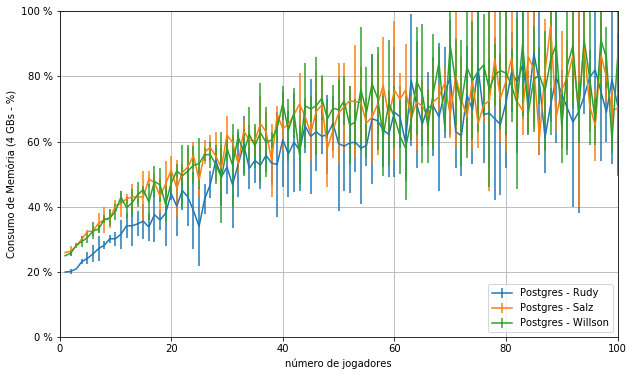
\includegraphics[width=0.8\textwidth]{figuras/analise/mem_db_media_por_jogador.png}
  \centering

  Fonte: O próprio autor.
\end{figure}

A partir da Figura~\ref{fig:mem_db_media_por_jogador} pode-se confirmar as conclusões parciais obtidas da Tabela~\ref{tab:cpu_db_media_quadrantes}.
%
Além das conclusões parciais, é possível visualizar o crescimento da média a cada incremento de jogador simultâneo.
%
pode-se concluir que o serviço de fato foi estressado, haja vista que pode-se perceber inicialmente um comportamento na qual não corresponde a uma curva multimodal.

A partir destes dados pode-se concluir que:

$$
    MEM(db\_postgresql_{r}) < MEM(db\_postgresql_{s}) \approx MEM(db\_postgresql_{w})
$$

Na qual entende-se:

\begin{itemize}
\item $MEM(db\_postgresql_{r})$: Curva de consumo de memória do PostgreSQL pela arquitetura Rudy;
\item $MEM(db\_postgresql_{s})$: Curva de consumo de memória do PostgreSQL pela arquitetura Salz; e
\item $MEM(db\_postgresql_{w})$: Curva de consumo de memória do PostgreSQL pela arquitetura Willson.
\end{itemize}
